\chapter{Comparisons: LightCycler 480 and QuantStudio 3/5}\label{ch:compare}

\section{What the temperature logs measure}
The demonstration treats the two temperature streams differently. These are generator assumptions, not calibration evidence:

\begin{itemize}
\item the \textbf{LightCycler 480} logs the \emph{block} temperature every 0.41\,s. Heating runs past the setpoint (overshoot
      of about 5\,°C at 95\,°C in the model), cooling undershoots, and the modelled peak ramp rates are
      (4.4--4.8\,°C/s heating, 2.2--2.5\,°C/s cooling);
\item the \textbf{QuantStudio 3/5} logs a \emph{modelled sample} temperature once per second. The model has no overshoot, ramps more
      slowly and depends on the block (96-well, 384-well, fast 0.1\,mL block).
\end{itemize}
Thermal numbers are therefore compared only within one instrument, and within one program (Chapter~\ref{ch:panel}).

\fig{cmp_thermal.png}{The first cycles of three synthetic runs aligned on the first cooling below 80\,°C: LightCycler block (blue) with overshoot and undershoot, QuantStudio 96-well sample model (red) and QuantStudio fast block (green, two-step 95/60\,°C program).}{cmp_thermal}

\begin{figure}[htbp]\centering
\begin{subfigure}{0.49\linewidth}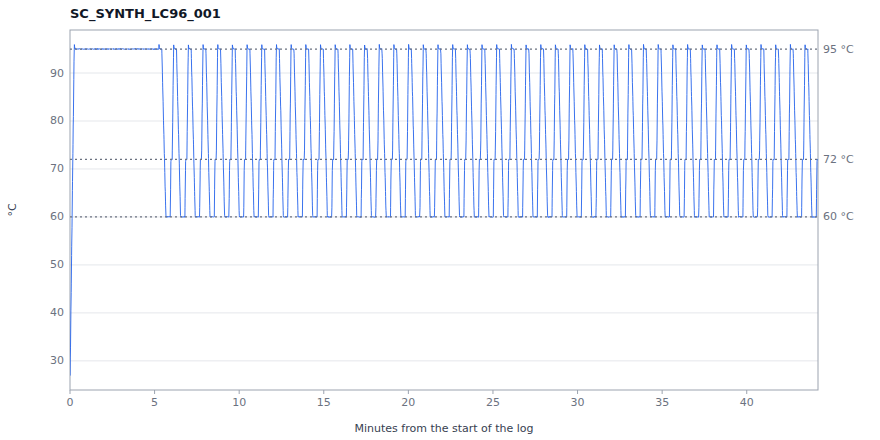
\includegraphics[width=\linewidth]{fig/g_LC_lc_thermal.png}\caption{LightCycler 480, block, 0.41\,s}\end{subfigure}\hfill
\begin{subfigure}{0.49\linewidth}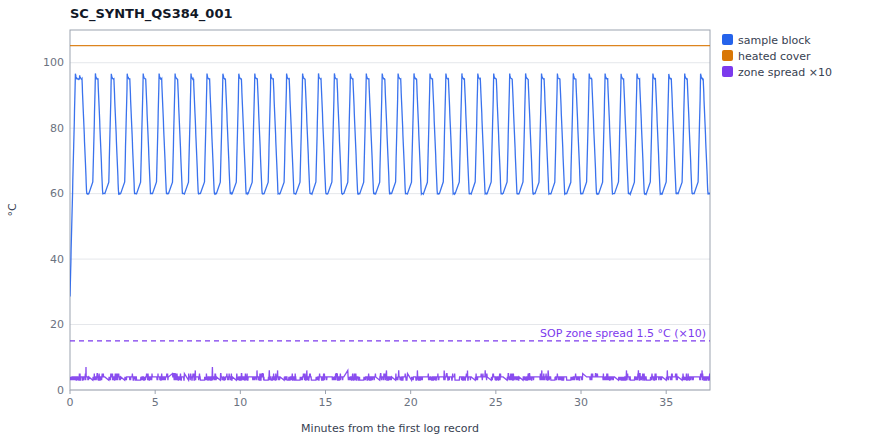
\includegraphics[width=\linewidth]{fig/g_QB_temperature.png}\caption{QuantStudio fast block, sample model, 1\,s}\end{subfigure}
\caption{\synthtag Whole-run temperature graphs of the two families side by side.}\label{fig:cmp_whole}
\end{figure}

\section{Instruments of the data set}
{\footnotesize
\begin{longtable}{@{}llllllll@{}}
\toprule \textbf{Column 1} & \textbf{Column 2} & \textbf{Column 3} & \textbf{Column 4} & \textbf{Column 5} & \textbf{Column 6} & \textbf{Column 7} & \textbf{Column 8} \\\midrule\endfirsthead
\toprule \textbf{Column 1} & \textbf{Column 2} & \textbf{Column 3} & \textbf{Column 4} & \textbf{Column 5} & \textbf{Column 6} & \textbf{Column 7} & \textbf{Column 8} \\\midrule\endhead
LC · LC-DEMO-01 & 180 & 4.85 & 2.43 & 14.5 & 5.8 & -0.484 & 97.6 \\\hline
LC · LC-DEMO-02 & 63 & 4.76 & 2.45 & 13.8 & 4.7 & -0.102 & 68.9 \\\hline
QS · QS-DEMO-A & 100 & 2.82 & 2.85 & 12.1 & 12.2 & – & 90.0 \\\hline
QS · QS-DEMO-B & 36 & 3.30 & 3.36 & 10.2 & 10.4 & – & 90.0 \\\hline
QS · QS-DEMO-C & 3 & 2.95 & 3.15 & 13.1 & 11.6 & – & 90.0 \\\hline
\bottomrule
\end{longtable}}



\begin{figure}[htbp]\centering
\begin{subfigure}{0.49\linewidth}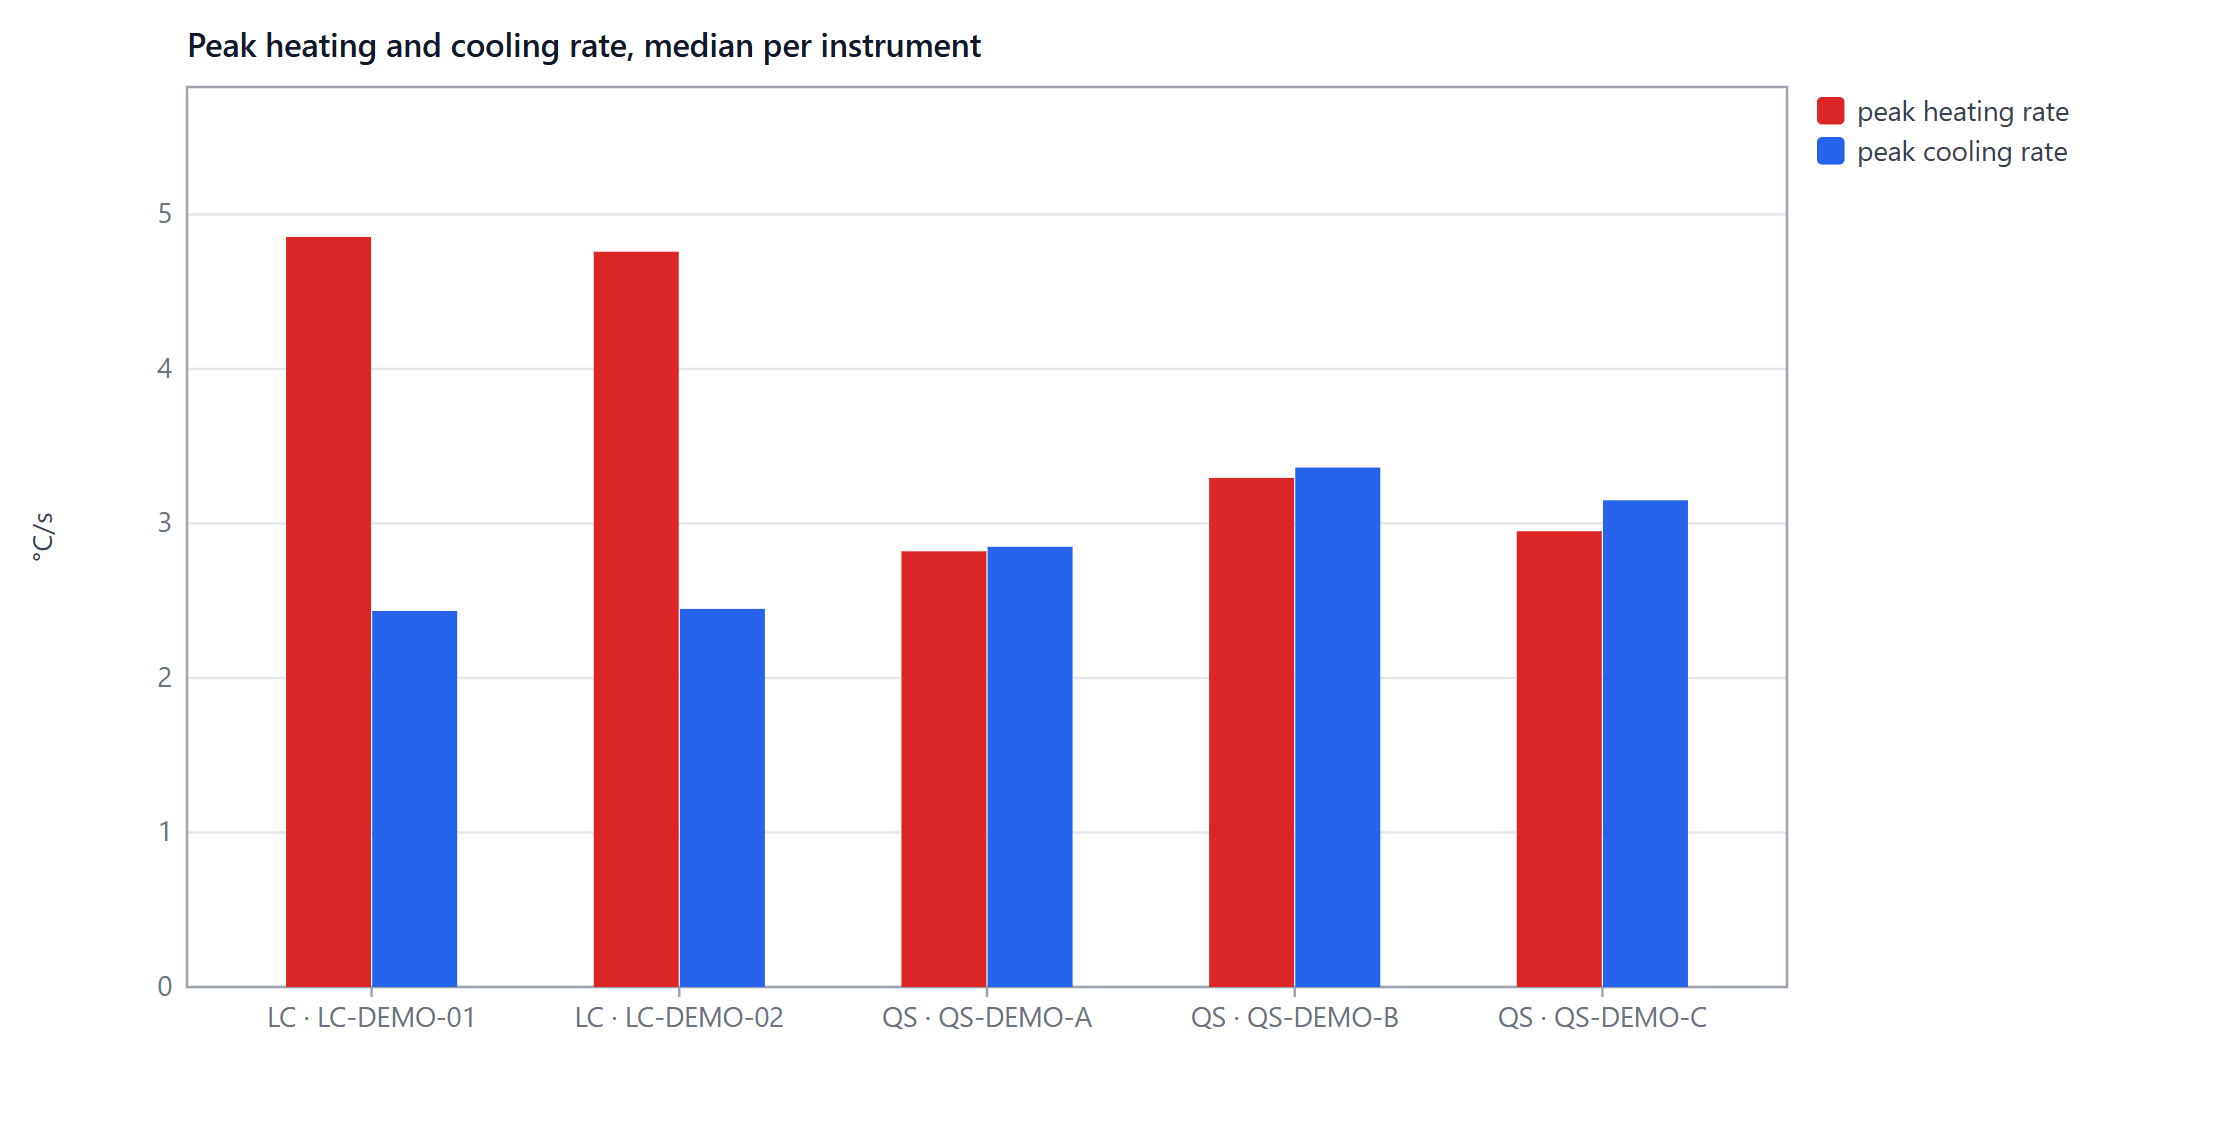
\includegraphics[width=\linewidth]{fig/cmp_rates.png}\caption{peak ramp rates}\end{subfigure}\hfill
\begin{subfigure}{0.49\linewidth}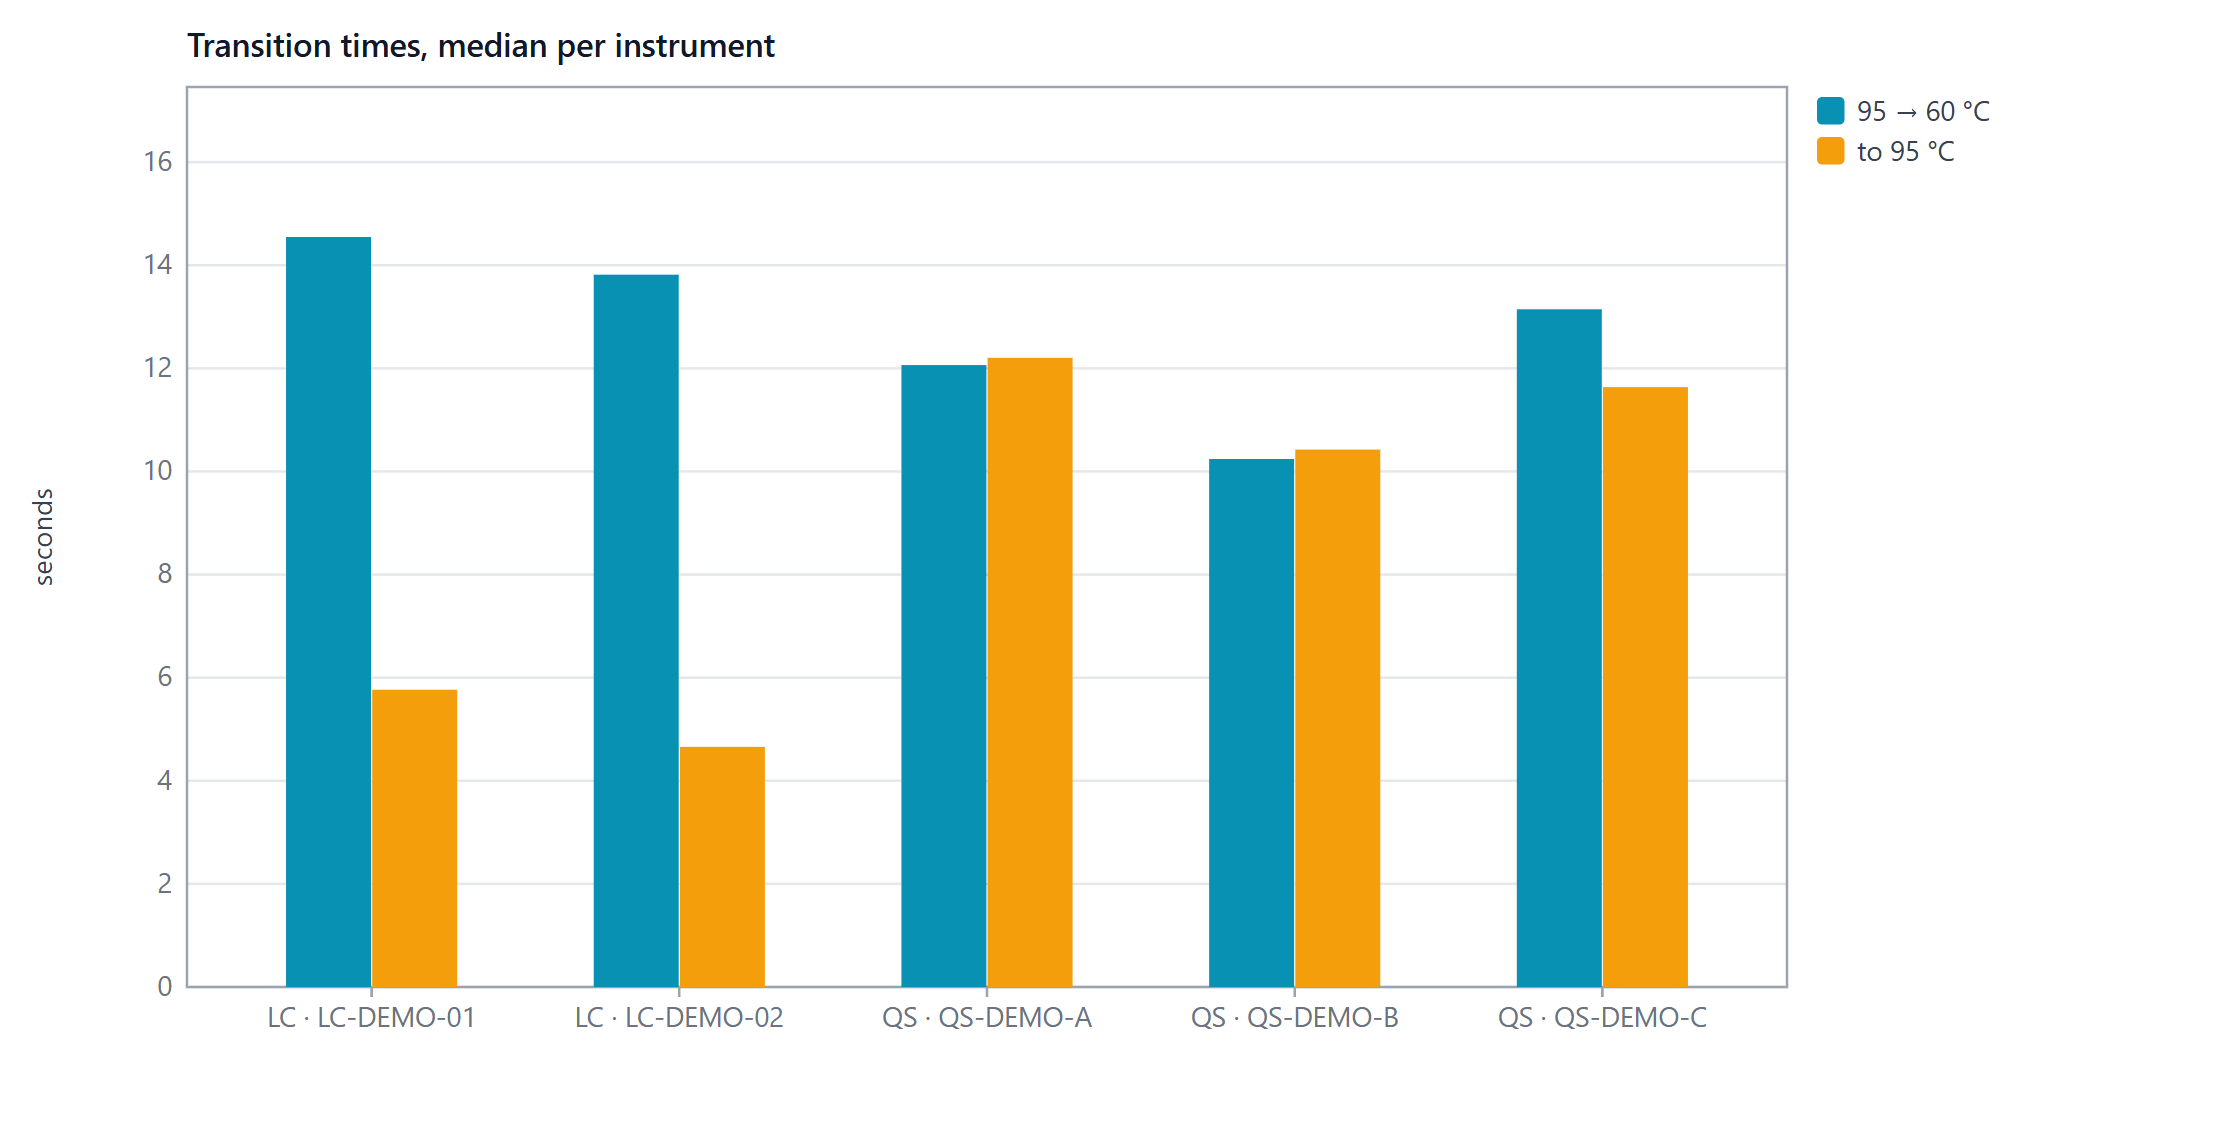
\includegraphics[width=\linewidth]{fig/cmp_transitions.png}\caption{transition times}\end{subfigure}
\caption{\synthtag Median peak heating and cooling rates and transition times per synthetic instrument. The LightCycler heats about twice as fast as it cools; the QuantStudio 96-well model cools faster than it heats because its program ramps are set lower than the block's maximum.}\label{fig:cmp_bars}
\end{figure}

\section{Stored and re-derived values}
Only the QuantStudio file stores $\Delta$Rn and the threshold, so only there can the page re-derive each Ct and compare it with the
stored one (Figure~\ref{fig:g_QS_recalc}). The LightCycler stores the crossing point of its own algorithm (second-derivative maximum
or fit points) with the raw fluorescence; the page reports it as stored and uses the curves for the plausibility checks
(end-point against Cq, unanalysed signal, copied curves).

\section{What each family contributes to the control panel}
\begin{center}\small
\begin{table}[H]\centering\small
\begin{table}[H]\centering\small
\begin{tabular}{|p{9cm}|p{3cm}|p{0.40\linewidth}|}

\hline
Chart family & LightCycler 480 & QuantStudio 3/5\\\hline
Ramp rates, overshoot, settling, transitions, reading temperature & block log & sample model\\ \hline
Zone uniformity, heat sink, heated cover & -- & yes\\ \hline
Lamp reference and drift / LED current and junction & lamp & LED\\ \hline
Exposure & automatic integration time & requested exposure\\ \hline
Filter wheel, encoder, camera, cover drive & channel switch only & yes\\ \hline
Embedded computer (replies, timer, scheduler, image processing) & -- & yes\\ \hline
Calibrations, saturation, block cycle counter & -- & yes\\ \hline
Data integrity, dates, method and operator charts & yes & yes\\\hline
\end{tabular}
\caption{Symbols of the area \emph{What each family contributes to the control panel}}
\end{table}
\caption{Symbols of the area \emph{What each family contributes to the control panel}}
\end{table}
\end{center}
